\documentclass[aspectratio=169,11pt]{beamer}

% ============================ theme & packages ============================
\usetheme{Boadilla}
\usecolortheme{seahorse}
\setbeamertemplate{navigation symbols}{}
\setbeamertemplate{itemize item}{\textbullet}
\setbeamertemplate{blocks}[rounded][shadow=false]

\usepackage[T1]{fontenc}
\usepackage[utf8]{inputenc}
\usepackage{lmodern}
\usepackage{amsmath,amssymb,bm}
\usepackage{xcolor}
\usepackage{tikz}
\usetikzlibrary{arrows.meta,positioning}

% ----- palette (matches docs/compositional_vae_slides.tex) -----
\definecolor{cSimplex}{HTML}{2563EB}  % DIVA beta-VAE   (blue)
\definecolor{cLik}{HTML}{C2410C}      % DIVA Hyp-PhILR  (orange)
\definecolor{cLatent}{HTML}{7C3AED}   % DIVA TreeDTM    (purple)
\definecolor{cAccent}{HTML}{BE185D}
\definecolor{cMuted}{HTML}{475569}

\newcommand{\ilr}{\operatorname{ilr}}
\newcommand{\clr}{\operatorname{clr}}

\tikzset{
  arrow/.style={-{Latex[length=1.6mm]}, semithick, draw=cMuted},
}

% tighter, calmer bullet lists inside the cards
\setbeamertemplate{itemize/enumerate body begin}{\scriptsize}

% uniform card body height so all three cards align to a shared baseline
\newcommand{\cardbodyH}{3.6cm}

\begin{document}

\begin{frame}{Three DIVA models --- domain-invariant VAEs at a glance}

  \begin{columns}[T]

  % --------------------------- DIVA beta-VAE ---------------------------
  \begin{column}{0.32\textwidth}
    {\setbeamercolor{block title}{fg=white,bg=cSimplex}%
     \setbeamercolor{block body}{bg=cSimplex!7}%
    \begin{block}{\centering DIVA $\beta$-VAE}
      \begin{minipage}[t][\cardbodyH][t]{\linewidth}
      \centering
      \begin{minipage}[c][1.3cm][c]{\linewidth}\centering
      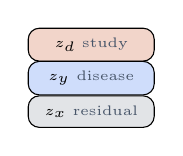
\begin{tikzpicture}[scale=0.85, every node/.style={font=\tiny}]
        \node[draw,rounded corners,fill=cLik!22,    minimum width=16mm,minimum height=4mm] at (0,0.9){$z_d$ \textcolor{cMuted}{study}};
        \node[draw,rounded corners,fill=cSimplex!22, minimum width=16mm,minimum height=4mm] at (0,0.4){$z_y$ \textcolor{cMuted}{disease}};
        \node[draw,rounded corners,fill=cMuted!16,   minimum width=16mm,minimum height=4mm] at (0,-0.1){$z_x$ \textcolor{cMuted}{residual}};
      \end{tikzpicture}
      \end{minipage}
      \par\smallskip
      \raggedright\footnotesize
      \emph{Split $\mathbf z$ into study, disease \& residual.}
      \begin{itemize}\setlength\itemsep{3pt}
        \item \textbf{Backbone:} Gaussian VAE on log-counts.
        \item Lightest variant --- ablation baseline.
      \end{itemize}
      \end{minipage}
    \end{block}}
  \end{column}

  % ------------------------ DIVA Hyp-PhILR-NB --------------------------
  \begin{column}{0.32\textwidth}
    {\setbeamercolor{block title}{fg=white,bg=cLik}%
     \setbeamercolor{block body}{bg=cLik!7}%
    \begin{block}{\centering DIVA Hyp-PhILR-NB}
      \begin{minipage}[t][\cardbodyH][t]{\linewidth}
      \centering
      \begin{minipage}[c][1.3cm][c]{\linewidth}\centering
      
\begin{tikzpicture}[scale=0.85, every node/.style={font=\tiny}]
        \draw[cLik,thick] (0,0.45) circle (0.6);
        \draw[cMuted,thin] (-0.42,0.72) to[bend left=35] (0.45,0.78);
        \fill[cLik]     (-0.18,0.5) circle (1.3pt);
        \fill[cSimplex] (0.28,0.22) circle (1.3pt);
        \fill[cMuted]   (0.08,0.82) circle (1.3pt);
        \node[cMuted] at (0,-0.4){Poincar\'e ball};
      \end{tikzpicture}
      \end{minipage}
      \par\smallskip
      \raggedright\footnotesize
      \emph{The same split, on the Poincar\'e ball.}
      \begin{itemize}\setlength\itemsep{3pt}
        \item \textbf{Backbone:} compositional PhILR (NB).
        \item Latent on the ball via $\exp_0$ map.
      \end{itemize}
      \end{minipage}
    \end{block}}
  \end{column}

  % ------------------------- DIVA TreeDTM-VAE --------------------------
  \begin{column}{0.32\textwidth}
    {\setbeamercolor{block title}{fg=white,bg=cLatent}%
     \setbeamercolor{block body}{bg=cLatent!7}%
    \begin{block}{\centering DIVA TreeDTM-VAE}
      \begin{minipage}[t][\cardbodyH][t]{\linewidth}
      \centering
      \begin{minipage}[c][1.3cm][c]{\linewidth}\centering
      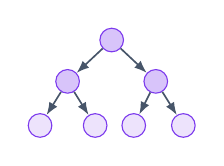
\begin{tikzpicture}[scale=0.7, every node/.style={font=\tiny},
        nd/.style={draw,circle,inner sep=0pt,minimum size=3mm,fill=cLatent!30,draw=cLatent},
        lf/.style={draw,circle,inner sep=0pt,minimum size=3mm,fill=cLatent!14,draw=cLatent}]
        \node[nd] (r) at (1.5,1.2){};
        \node[nd] (a) at (0.7,0.45){};
        \node[nd] (b) at (2.3,0.45){};
        \node[lf] (l1) at (0.2,-0.35){};
        \node[lf] (l2) at (1.2,-0.35){};
        \node[lf] (l3) at (1.9,-0.35){};
        \node[lf] (l4) at (2.8,-0.35){};
        \draw[arrow](r)--(a); \draw[arrow](r)--(b);
        \draw[arrow](a)--(l1); \draw[arrow](a)--(l2);
        \draw[arrow](b)--(l3); \draw[arrow](b)--(l4);
      \end{tikzpicture}
      \end{minipage}
      \par\smallskip
      \raggedright\footnotesize
      \emph{The same split, with a tree likelihood.}
      \begin{itemize}\setlength\itemsep{3pt}
        \item \textbf{Backbone:} Dirichlet-tree-multinomial.
        \item Sibling-centred log-ratio encoder.
      \end{itemize}
      \end{minipage}
    \end{block}}
  \end{column}

  \end{columns}

  \vfill
  {\setbeamercolor{sharedband}{bg=cMuted!8,fg=cMuted}%
  \begin{center}
  \begin{beamercolorbox}[wd=0.985\textwidth,sep=5pt,center,rounded=true,shadow=false]{sharedband}
  \footnotesize Shared DIVA mechanism: latent split $\mathbf z=[z_d;z_y;z_x]$\,$\cdot$\,
  conditional priors $p(z_d\!\mid\!\text{study})$, $p(z_y\!\mid\!\text{disease})$\,$\cdot$\,
  aux.\ heads $q(d\!\mid\!z_d),\,q(y\!\mid\!z_y)$\,$\cdot$\, predict from $z_y$ only.
  \end{beamercolorbox}
  \end{center}}

\end{frame}

\end{document}
